\chapter{Религия}

\section{Научный атеизм: верить, не верить, как проверить?}

\textit{Источник: \url{https://4brain.ru/blog/nauchnyj-ateizm-verit-ne-verit-kak-proverit/}}

А давайте перенесемся в будущее, примерно в 2050 год, и попытаемся представить, как будут проходить уроки физики в школе через пару-тройку десятков лет? «Как идет ток по проводам? – С Божьей помощью! – Садись, пять!» Такой диалог ученика и учителя видится вполне реальным даже намного раньше, чем в 2050 году.

Разумеется, если только к этому времени физику не исключат из списка обязательных для изучения в школе предметов. После приказа Министерства просвещения, коим из перечня обязательных исключены астрономия, экономика, экология и право, удивляться не приходится ничему [Официальный интернет-портал правовой информации, 2022].

В том числе тому, что ракеты падают, вместо того, чтобы лететь, куда их направили. Взлетела, ударилась о небесный свод, упала, куда придется – что здесь непонятного? Так, видимо, будут объяснять все недоработки ракетной промышленности в обозримом будущем, когда знания по астрономии окончательно перейдут в категорию рудиментарных.

Наших читателей, уже прошедших программы «Критическое мышление» и «Когнитивистика», вряд ли чем-то можно сбить с толку. Мы приглашаем всех желающих присоединиться к нашему образовательному марафону, изучать наши программы и читать наши статьи. И наша сегодняшняя тема – научный атеизм.

\textbf{Что такое «научный атеизм»?}

Согласно существующему определению, научный атеизм – это система научно-материали- стических взглядов, основанная на полном отрицании существования Бога и прочих сверхъестественных сил.

Наличие явлений, не поддающихся трактовке с позиций науки, научный атеизм объясняет недостаточным уровнем развития научных знаний, который, впрочем, постоянно растет.

Следовательно, со временем все не вполне понятные на сегодняшний день явления будут изучены, поняты и все это без необходимости привлечения Божественных и других сверхъестественных субстанций.

\textbf{Научный атеизм: небольшой исторический экскурс}

Слово «атеизм» пришло к нам из далекой Античности. В древнегреческом языке слово atheos (читается как «атеос») означает «безбожный». Как мы понимаем, коль скоро слово с таким значением появилось в языке, значит, в социуме существовало такое явление, и возникла необходимость каким-то образом отобразить это в существующей системе обмена информацией.

Из известных мыслителей прошлых веков до нашей эры в существовании Бога очень сомневался Протагор (490-420), а Диагор Мелосский (475-410) и Феодор Киренский (340-250) прямо отрицали существование Бога. Термин atheismos («атеизм») использовал в своих работах Цицерон (106-43). С развитием научных знаний стали предприниматься попытки обосновать атеистические воззрения с научной точки зрения. Так зародилось понятие «научный атеизм».

Проследить эволюцию этого термина можно в книге Histoire de la littérature ancienne et moderne («История древней и современной литературы»), впервые изданной в 1829 году и восстановленной и переизданной уже в наступившем третьем тысячелетии [F. Schlegel, W. Duckett, 2011]. Уточним, с древних времен дошло не так много литературных источников, и в 19 веке древнюю литературу изучали без жесткого разделения на художественную и философскую.

В странах Западной Европы научный атеизм в большей степени приобрел форму научного скептицизма – подхода, согласно которому, все утверждения, которые не могут быть доказаны опытным путем, должны быть подвергнуты сомнению. А вот в нашей стране научный атеизм стал орудием идеологической борьбы, пропаганды и обработки массового сознания в нужном для партии направлении.

Да, в нашей стране риторика атеизма обязана своей распространенностью, массовым использованием и частым употреблением партийным лидерам ушедшей эпохи. Владимир Ленин, «вождь мирового пролетариата», создатель Российской социал-демократической рабочей партии (сокращенно РСДРП), впоследствии трансформировавшейся в РКП(б), ВКП(б) и затем в КПСС, рассматривал атеистическое воспитание как необходимую составляющую построения нового общества.

Его научные работы многократно переиздавались уже после его смерти, в частности, в виде сборника статей об атеизме, религии и церкви [В. Ленин, 1980]. В этих работах можно проследить формирование начал теории отражения и научного атеизма. Ленин писал, что отражение в сознании, образ представляет собой органическое единство непосредственного восприятия и прошлых впечатлений, объективного и субъективного, формы и содержания. В его понимании теория отражения как бы «соединяет» познающий субъект с познаваемым объектом и обеспечивает объективность научного познания, поэтому никакой необходимости в «божественном» объяснении окружающего мира не существует.

Собственно термин «научный атеизм» в СССР обрел популярность с началом правления Никиты Хрущева. Одно за другим вышли постановления «О крупных недостатках в научно-атеистической пропаганде и мерах по ее улучшению» и «Об ошибках в проведении научно-атеистической пропаганды среди населения». Уточним, что ранее в партийных руководящих документах использовался термин «антирелигиозная пропаганда», и лишь в 50-е годы было решено отказаться от противопоставления посредством приставки «анти» в пользу термина «научно-атеистическая пропаганда».

С 1959 года в высших учебных заведениях начали преподавать «Основы научного атеизма», сначала факультативно и не везде [М. Смирнов, 2018]. Но дело быстро набирало обороты, и уже в 1960 году научный атеизм в МГУ преподавали на всех факультетах. За столицей «подтянулась» вся страна, практически во всех вузах появилась кафедра научного атеизма. Появилась и соответствующая учебная литература. В частности, «Научный атеизм» учебник СССР для высших учебных заведений [А. Окулов, 1978].

В 1964 году был создан Институт научного атеизма, просуществовавший вплоть до развала СССР и еще какое-то время в уже переименованном виде как Институт религиоведения. Институт научного атеизма на протяжении почти всего своего времени существования выпускал сборник «Вопросы научного атеизма», в задачи которого, как было заявлено, входила разработка актуальных проблем теории и практики научного атеизма, анализ и обобщение опыта научно-атеистического воспитания.

Под эгидой общества «Знание» в рамках проекта «Новое в жизни, науке, технике» издавалась подписная научно-популярная серия «Научный атеизм» с упором в большей степени на историю и философию. В рамках этой серии вышла, к примеру, очень познавательная книга «Атеистические традиции в русской философии» [А. Сухов, 1989].

Показательно, что советские разработки в этом направлении вызывали определенный интерес в научных кругах на Западе. Так, в периодическом издании Studies in Soviet Thought («Исследования советской мысли») вышла статья Scientific Atheism: An Introduction («Научный атеизм: введение») [T. Blakeley, 1964].

Позднее вышла еще одна статья этого же автора под названием Marxist‐Leninist scientific atheism («Марксистско-ленинский научный атеизм») [T. Blakeley, 1966]. Автор делится своими выводами, что в его понимании главная цель марксистско-ленинского «научного атеизма» состоит в открытии и усвоении «научных» данных и использовании их в «атеистическом» уничтожении религии и всех ее придатков. Первая задача состоит в том, чтобы показать, используя данные преимущественно естественных наук, отсутствие объекта религии – Бога. Во-вторых, «научный атеизм» стремится объяснить, как возникла и продолжает проявлять признаки жизнестойкости теория без объекта, ищет причины или «корни» религии.

В нашей стране печатные издания на тему атеизма «сошли на нет» еще до распада Советского Союза. Было ли дело только в невостребованности и неактуальности темы в новых условиях перестройки и гласности или решающую роль сыграла нехватка финансирования, мы сейчас не узнаем. С учетом того, что в конце 80-начале 90-х недофинансирование ощущали даже весьма важные для обороноспособности страны отрасли, можно предположить, что финансовый фактор стал решающим.

Однако и тему востребованности тоже нельзя сбрасывать со счетов. Когда появляется актуальный запрос, находятся и ресурсы для его реализации. Примером может служить книга Устина Чащихина «Научный атеизм» (скачать можно здесь) вышедшая в 2013 году спустя более чем 20 лет после того, как Советский Союз канул в Лету. А в 2022 году вышла новая книга, которую написал Устин Чащихин «Научный атеизм – спасение России».

Что это за актуальность такая с учетом того, что в российских школах уже давно преподается Закон Божий под красивым названием «Основы православной культуры»? А вот об этом стоит поговорить подробнее.

\textbf{Научный атеизм сегодня: актуально или нет?}

На самом деле, поводов обратить взор в сторону научного атеизма сегодня более чем достаточно. Судите сами: церквями и храмами у нас застроили все вокруг, детишек сызмальства заставляют изучать Закон Божий, сами все молимся и крестимся, чуть ли не двумя руками, а живем все хуже и хуже. И ладно бы дело было только в материальной составляющей.

Зла и ненависти стало вокруг намного больше, невзирая на то, что религии и морали, вроде как, все пути к нашим сердцам открыты. А заповедь «Не убий», такое впечатление, что все просто позабыли и действуют строго наоборот, особенно в 2022 году.

Люди постарше вполне могут вспомнить, что в эпоху марксизма-ленинизма, научного атеизма и научного коммунизма военные конфликты, если и возникали, решались исключительно \ed{усилиями}{усилие}{effort} действующей армии и без особой \ed{огласки}{огласка}{publicity}. Митинги и демонстрации были исключительно праздничные, приуроченные к различным «красным дням календаря» и, естественно, санкционированные властью.

И, что характерно, особых поводов хотя бы задуматься о несанкционированном митинге протеста не было. Это не к тому, что «раньше было лучше», а к тому, что с проблемами, которые есть всегда и в любом государстве, каким-то образом справлялись так, чтобы не нарушать покой «широких народных масс».

Так может, если перестать молиться и начать думать, а вместо храмов и церквей строить школы и университеты, все как-то наладится? Знать это однозначно и заранее невозможно, однако повод задуматься, безусловно, есть.

Ранее упомянутая нами книга «Научный атеизм» начинается с той ценной мысли, что, если Бог не может уничтожить зло, значит, он не всемогущ, а если не хочет, то его доброта, мягко говоря, сильно преувеличена [У. Чащихин, 2013].

Если же Бог не может и не хочет уничтожить зло, тогда зачем он вообще такой нужен? Эту мысль когда-то высказал древнегреческий философ Эпикур (342-271), однако тема актуальна по сей день. Видимо, за добротой и \ed{человеколюбием}{человеколюбие}{philanthropy} – это точно не в церковь.

Вышеупомянутое издание «Научный атеизм» – книга, которая содержит много отсылок к историческому материалу. Автор очень настаивает на том, чтобы люди, считающие себя верующими, внимательно прочитали «Ветхий Завет» и «Новый Завет» и задумались, что именно они взяли за образец в своей жизни.

Все подряд цитировать не будем, однако то, что в библейской литературе много чего такого, что к доброте и человеколюбию не имеет никакого отношения, это факт. Просто цитата: «И послал тебя Господь в путь, сказав: иди и предай заклятию нечестивых Амаликитян и воюй против них, \explain{доколе не уничтожишь их}{until you destroy them}» [allbible, 2015].

При всем понимании, что у каждой фразы есть свой контекст, сложно смириться, что призыв решить проблему военным путем \explain{из уст}{from the mouth} Господа – это нормально. Так что религия – это не так однозначно хорошо, как это пытаются внушить на уровне государства, которое, вроде как, отделено от церкви.

Почему тогда научный атеизм времен СССР так и не прижился в массовом сознании, невзирая на то, что его преподавали в вузах, пропагандировали посредством научно-популярной литературы, а ночному пасхальному богослужению всегда предлагали более \ed{зажигательную}{зажигательная}{incendiary} альтернативу – концерт Аллы Пугачевой и других звезд \ed{эстрады}{эстрада}{stage} по центральному телевидению?

Автор книги «Научный атеизм» объясняет это не слишком высоким профессиональным уровнем тогдашней научно-атеистической пропаганды [У. Чащихин, 2013]. По сути, тогда в подготовке материалов по научному атеизму в полную силу участвовали представители только одной науки – философии, а аргументы из естественных наук были на уровне школьных учебников физики, географии и биологии.

Сам автор явно гордится тем, что он не гуманитарий, а представитель естественных наук, что уже само по себе должно обеспечить более современную и «\ed{продвинутую}{продвинутая}{advanced}» аргументацию. Зачем нужна эта аргументация и зачем в принципе опять поднимать на щит вопросы научного атеизма?

А вот с этого момента появляется ощущение, что где-то мы уже это все видели, слышали, читали и проходили. Ответ на вопрос «Зачем нужен научный атеизм» сводится к следующим постулатам:
\begin{enumerate}
    \item Научный атеизм развивает научное мышление.
    \item Научный атеизм экономит время, которые верующие тратят на молитвы и посещение церкви.
    \item Научный атеизм экономит денежные средства, которые верующие тратят на покупку церковной атрибутики.
    \item Научный атеизм прекращает религиозные войны и религиозную ненависть.
\end{enumerate}

\ed{Насчет}{насчёт}{as regards} последнего можно поразмыслить. Быть может, если дать «ИГИЛовцам» (признана в РФ экстремистской организацией) почитать книжки по научному атеизму, что-то и изменится. А вот насчет экономии времени и денег – вряд ли это станет весомым аргументом, который может сподвигнуть верующих отказаться от веры и соблюдения церковных ритуалов. Эти же аргументы – экономия времени и денег – можно выдвинуть желающим «собраться с ребятами на пиво», «сходить с девочками попить кофе», «поехать порыбачить на русалок» и т.д.

Гипотетически в этой жизни можно не тратиться ни на что, кроме еды, жилья, одежды и средств гигиены, только что это будет за жизнь? Прихожане любой церкви – это почти как участники группы по интересам, где у каждого своя интенсивность участия в общем деле. Кто-то посещает церковь по всем праздникам, скупает все свечки, причащается и исповедуется, а кто-то приходить лишь на Рождество и Пасху и довольствуется ролью зрителя.

Так за что же борется или «против кого дружит» научный атеизм? То, что Бог, даже если он есть, не всесилен и не может решить проблемы людей без их участия понятно даже глубоко верующим. Как говорится, батюшка в бронежилете и бронированном джипе – наглядное подтверждение известной поговорки «На Бога надейся, а сам не плошай».

\begin{center}
    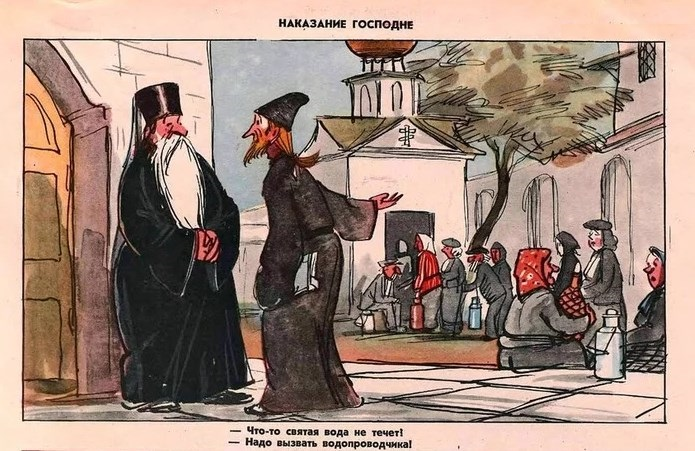
\includegraphics[width=0.8\textwidth]{img/holy-water.jpg}
\end{center}

Так ли далеко от этого ушел научный атеизм – карикатуры, которые использовались для научно-атеистической пропаганды, говорят об обратном. Например, для того, чтобы святая вода исправно поступала верующим, нужен исправно работающий водовод, а для того чтобы его отремонтировать, нужен водопроводчик.



Есть и еще одна вариация на эту тему, когда заболевший священнослужитель обращается со словами «Помоги, Господи» к аптекарю, а не собственно к Богу.

Что и чему здесь противоречит? Маловероятно, что священнослужители возьмутся оспаривать необходимость вызвать сантехника, если сломался водовод, или обратиться к врачу в случае болезни, потому как «На Бога надейся, а сам не плошай». Или вот такой опус:

\begin{fancyquotes}
    У церковного порога ждешь, поп, напрасно:\\
    Без икон и Бога мы живем прекрасно!
\end{fancyquotes}

Как говорится, слава Богу, что кто-то может решить свои проблемы своими силами и не беспокоить Всевышнего всякими мелочами:

\begin{wrapfigure}{l}{0.5\textwidth}
    
\includegraphics[width=0.5\textwidth]{img/atheism-church.jpg}
\end{wrapfigure}
Иначе может получиться, как в анекдоте, когда глубоко верующий попал и постоянно молившийся прихожанин в ад, а крепко пьющий столяр-безбожник – в рай. На вопрос верующего «Почему?» последовал вполне логичный ответ, что где это видано, чтобы табуретки бегали за столяром и «доставали» его своими проблемами.

\begin{wrapfigure}{r}{0.5\textwidth}
    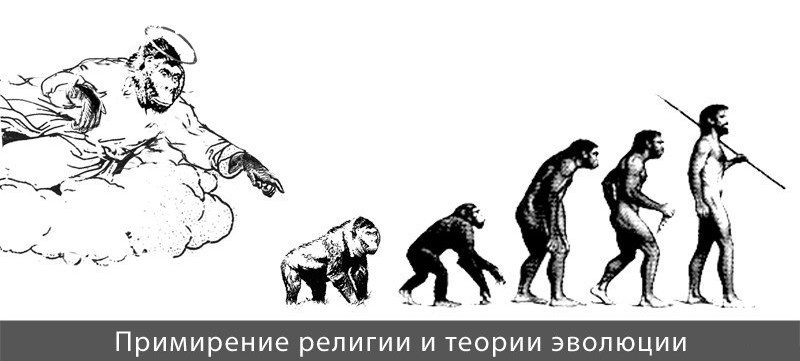
\includegraphics[width=0.5\textwidth]{img/atheism-monkey.jpg}
\end{wrapfigure}
Были, правда, и попытки «примирения» науки и религии, к примеру, по вопросу о происхождении человека. С учетом того, что живьем Бога все равно никто не видел, допущения могут быть абсолютно любые. Насколько удачные – судите сами.
Однако самой фееричной на тему научного атеизма карикатурой можно считать, пожалуй, ту, где студентка молится Богу, чтобы сдать научный атеизм:

Как говорится, «кафедра научного атеизма в шоке», но кого это волнует, когда «на кону» стипендия.

Так или иначе, и в религиозной, и в научно-атеистической пропаганде можно найти какие-то изъяны. Однако есть ученые, которые занимаются критикой научного атеизма профессионально и получают за это зарплату.\\


\textbf{Критика научного атеизма}

Сегодня в обществе существует запрос на сохранение баланса между верой и знанием, светским и религиозным, охрану личных границ от вмешательства какой-либо идеологии со стороны будь то церкви или государства. Именно этим и обусловлены циклические всплески интереса к вопросам научного атеизма.

Однако у определенной группы ученых есть большие сомнения, что научный атеизм может решить эту задачу и что в принципе в ныне существующем виде научный атеизм имеет право называться научным. Так, в статье The reasons for «scientific» atheism (Причины «научного» атеизма) можно найти витиеватую мысль насчет того, что «научный атеизм противоречит сам себе, потому что, если бы он был правдой, ему не пришлось бы трудиться, чтобы опровергнуть иллюзию» [J. Cañizares, 2012].

Стоит ли это понимать так, что если бы география была правдой, так ей бы не пришлось опровергать иллюзию многих поколений людей, что Земля плоская? А если бы правдой была химия, то ей не пришлось бы опровергать иллюзию божественного происхождения молекул и атомов, и в химических формулах и таблице Менделеева не было бы никакой необходимости? Как говорится, «не совсем понятно».

\begin{wrapfigure}{l}{0.5\textwidth}
    
\includegraphics[width=0.48\textwidth]{img/atheism-4.jpg}
\end{wrapfigure}
Есть и более здравые мысли. Бразильский физик-теоретик Марсело Глейзер в своем интервью по поводу получения Темплтоновской премии 2019 года заявил, что «отсутствие доказательств не является доказательством отсутствия», и именно поэтому «атеизм несовместим с научным методом» [L. Billings, 2019].

Насчет того, что «отсутствие доказательств не является доказательством отсутствия», с этим нужно полностью согласиться. Однако само по себе «отсутствие доказательств отсутствия» не может автоматически считаться доказательством присутствия. В этом плане атеизм полностью следует в русле формы научного скептицизма – подхода, согласно которому, все утверждения, которые не могут быть доказаны опытным путем, должны быть подвергнуты сомнению.

Всем, кому хочется больше критики, можем порекомендовать статью «Сердце бессердечного мира: Как родился и умер советский научный атеизм» [А. Коняев, А. Артемьев, 2013]. Мы долго останавливаться на критических замечаниях не будем ввиду однотипности предлагаемых критиками аргументов и бессмысленности критики всего, что в какой-то момент времени оказалось востребованным и отвечающим запросам текущей ситуации.

В конце концов, религия – это не только идеология, которую можно принимать или не принимать, критиковать или продвигать в массы. Это красивые обряды, это душевные песнопения, это самобытная архитектура церквей. Это еще несколько праздников в наш насыщенный трудовыми буднями календарь, это возможность отдохнуть душой, отмечая вместе с близкими людьми, к примеру, Пасху.

Подготовка к этому празднеству столь же замечательна, как и само празднование: покраска яиц всей семьей, выбор узоров и красящих субстанций, эксклюзивные сюжеты и стандартные трафареты, которые нужно максимально гармонично разместить на поверхности яйца. А в день Пасхи по традиции принято устраивать «сражения», по очереди ударяя друг о друга окрашенные куриные яйца и выясняя, с какой стороны скорлупа крепче: с более округлой или с более заостренной.

Большинство людей, отмечающих Пасху и красящих куриные яйца, не читали Библию и не считают для себя обязательным посещение церкви. Стоит ли им мешать просто наслаждаться жизнью, праздниками, общением и застольем, досаждая всяческими опусами на тему научного атеизма и ненужности религии как таковой?

Думается, вряд ли, потому что у нас уже была страна, которая пыталась запрещать людям совершать церковные обряды, крестить детей и венчаться, праздновать Пасху, читать Солженицына и Довлатова, слушать «Битлз» и ДДТ. Страна называлась СССР, и ее больше нет, в то время как книги Солженицына и Довлатова читают до сих пор, «Битлз» и ДДТ как слушали, так и слушают, а Пасху как отмечали, так и будут отмечать дальше все, кто считает это нужным для себя.

Закончит так же плохо, как СССР, любая другая страна, которая будет запрещать, ограничивать и убеждать людей в том, что им не нужно многое из того, к чему они привыкли? Мы не знаем, но проверять не хотелось бы. А хотелось бы, чтобы в нашу жизнь вернулся мир, добро и взаимопонимание, причем совершенно не важно, как: через религию, науку или атеизм.

\newpage
\section{Язык и религия}

\textit{Источник: \url{https://4brain.ru/blog/jazyk-i-religija/}}
Религию можно обозначать в любых категориях – ее называют системой верований, идеологией, «опиумом», неосознанным и трансцендентальным знанием об окружающем мире. В любом виде она представляет сначала систему идей, концепций, ассоциаций и сравнений, которые могут переноситься людьми в материальную культуру.

Но, независимо от категорий, важно понимать одно: религия без слов, общего языка и системы мышления не сможет существовать больше одного поколения. Религия – это совокупность неких абстрактных смыслов, которые можно передать при помощи слов, языка.

В идеализированном понимании религия не предусматривает необходимости защищать себя от скептиков или же искать самой себе подтверждения – передачи знания и религиозных основ от поколения к поколению было бы достаточно, чтобы последователи поддерживали религию живой. Подходящей цитатой в этом случае является цитата Джалаладдин Руми (Sufi mystic Rumi): «Тишина – это язык Бога».

Но с другой стороны, исторически становится очевидным, что язык как средство сохранения религии является также и главной причиной, почему религиозные знания не могут передаваться дословно, точно, без интерпретаций, скептицизма и дискурсивности. Именно создавая новые интерпретации той или иной догмы, множество скептиков или реформистов создавали новую религию.

Таким образом, вопрос связи языка и религии – это нечто больше, чем сохранение культурной традиции. Язык и религия вызывают интерес разных мыслителей и ученых на протяжении столетий, начиная со времен Аристотеля и заканчивая сегодняшним днем (больше о последних исследованиях можно почитать в нашей статье «Язык и мышление»).

\textbf{Обозначение взаимозависимости}

С философской точки зрения, язык и религия – это два инструмента человеческого сознания, которые помогают объяснить организацию внешнего мира, создать ощущение общности. Поэтому религия и язык являются такими же формами сознания, как философия, мораль, право, искусство и наука, ибо все они преследуют единую цель – отображать мир в сознании человека.

Поскольку язык и религия – это два разных подхода к пониманию мира, для более четкого обозначения предмета дискуссии их используют вместе, как понятие «язык и религия». Это придает новое значение данным понятиям и позволяет рассматривать их наряду с другими стойкими философскими категориями, такими как «язык и общество», «язык и сознание», «язык и культура».

Но все-таки очевидным можно назвать то утверждение, что религия является более зависимой от языка. Именно при помощи языка создаются и сохраняются все религиозные образы, что делает психологические структуры языка и религии между собой тесно сплетёнными.

\textbf{Вильгельм фон Гумбольдт и «дух народа»}

Интерес к изучению истории и духа (культуры) европейских народов был заложен философом Вильгельмом фон Гумбольдтом. Вслед за философией Гегеля, который провозгласил идею «духа народа» неотъемлемой составной частью человеческого бытия, Гумбольдт развил направление сравнительной антропологии, которое интересовалось историей, бытом, фольклором и, конечно же, религией – важными составными чертами народов.

Непосредственно Гумбольдт также предположил, что язык возник как результат духовного развития народа, и это нечто большее, чем общественное сознание, – это различное видение мира. К такому заключению он пришел во время изучения языка басков, который разительно отличался от языков своей индоевропейской семьи. В своей работе «О различии строения человеческих языков и его влиянии на духовное развитие человечества» Гумбольдт описывал непосредственное влияние языка на формирование духовного сознания человека.

\textbf{Сакрализация текстов и их роль}

Наивысшей формой развития духовного сознания некой общности людей является создание собственных сакральных книг – Торы, Священного Писания, Корана, Авесты, проповедей Будды. Каждый из этих текстов стал чем-то большим, нежели просто послужил формированию народной общности, – со временем приверженцы той или иной религии не ограничивались географическими границами, могли сохранять чувство единения с единомышленниками независимо от местонахождения. Такое чувство общности оказалось даже более стойким в формировании ментального родства, чем использование одного языка, на котором тексты были написаны.

Таким образом, независимо от религии и языка, на котором передаются сакральные знания, язык и религия все равно являются важными элементами человеческого познания и объяснением мироустройства, роли человеческой жизни и жизни после смерти.

Другая важная особенность сакральных текстов состоит в том, что вокруг них формируется целая прослойка важных культурных и духовных проявлений приверженцев – особое религиозное мироощущение, традиции, обряды, религиозная мораль, религиозные институты. Все эти материальные проявления абстрактной религии делают более четкими и понятными духовную практику для многих последователей вне национальных ограничений.

\textbf{Атеистический экзистенциализм: возможна ли жизнь без Бога}

Несмотря на силу религиозного учения и его интерпретации общественного строя, другим проявлением человеческого сознания является полное или частичное отрицание божественной, мифической и духовной потребности человека в Боге в любой форме – трансцендентальной, метафизической и религиозной. Приверженцы этого философского направления – атеистического экзистенциализма (Жан-Поль Сартр, Альбер Камю, Мартин Хайдеггер и Симона де Бовуар), опровергая большинство принятых христианских канонов, не смогли выйти из религиозной перспективы мира, ибо заявили о реинкарнации как форме спасения.

\textbf{Религиозная практика сегодня}

В современном мире, транскультурные границы которого все больше и больше теряют свое значение, святость религиозного языка выглядит, как последний не тлеющий бастион. Особенно в мегаполисах или в далеких странах религия и язык часто являются самыми важными атрибутами национального и культурного единства. Молитва на родном языке сохраняет ощущение единства с культурой и историей.

В современном глобальном мире, где люди часто теряют свои корни и помнят о них из детских рассказов, изучение родного языка и молитва на нем выполняют важную практику духовного воссоединения со своими корнями. Такая тенденция наиболее популярна среди современного еврейского населения, часть которого проживает в разных странах мира. Именно язык и религия являются источниками воссоединения с прошлым. Для них иврит – это интимный способ понимания своей религии, культуры и философии в более точных понятиях. Таким образом, независимо от контекста, именно использование религиозных терминов в ежедневном лексиконе, вместе с отмечанием праздников, помогает осмысливать свое существование и историю.

С другой стороны, разнообразный исламский мир именно при помощи религиозного языка и канонов веры сохраняет свое ощущение единства – из 5 разновидностей арабского языка сиро-палестинский диалект (Levantine Arabic) – самый универсальный, и на этом диалекте написан Коран, поэтому он понятен большинству арабов.

И более того, язык религии может не только поддерживать существование национальной культуры, где бы ее последователи ни обитали, – он может создавать новые общества, объединяя разных людей. Именно такой необычный путь свойственен классическому тибетскому языку. Его первые последователи появились в Британии в 1960-х гг., где учредили монастырь и стали объединять всех желающих изучать буддизм.

\textbf{Вместо заключения}

Язык и религия как мировоззрение являются проявлением человеческого сознания, и, независимо от трансформаций, служат неотъемлемым способами познания мира человеком. Их роль заключается в более сложной функции, чем роль общественного или политического мировоззрения, ибо при помощи религии и языка человечество пытается не столько обустроить свою жизнь, сколько найти ответы на вопросы о своем существовании.


\newpage
\section{Бог изменил мою жизнь}

\textit{Как порнозвезда из 2000-х отказалась от миллионов и стала проповедницей?}

\textit{Источник: \url{https://lenta.ru/articles/2023/10/21/delamora/}}

В нулевых годах порноактриса Бриттни Де Ла Мора, известная под псевдонимом Дженна Пресли, была настоящей суперзвездой. За семь лет работы модель снялась примерно в 300 порнографических сценах. Она зарабатывала десятки тысяч долларов в месяц, водила дорогие автомобили и носила одежду \ed{люксовых}{люксовый}{luxury} брендов. Но в ее жизни была и другая сторона. Изнасилование, зависимость от наркотиков, анорексия, \ex{половые заболевания}{sexual diseases} --- через все это пришлось пройти Де Ла Море, прежде чем она смогла изменить свою жизнь. Как она отказалась от многомиллионных гонораров, вышла замуж за пастора и вместе с ним начала \ex{проповедовать в церкви}{to preach in church} --- в материале «Ленты.ру».

\textbf{«Иисус любит порнозвезд».} «Я очень горжусь тем, как изменилась моя жена. Она была совершенно потерянной, а теперь она нашла свое место», --- так пастор Ричард Де Ла Мора говорил о своей супруге Бриттни.

Впервые Де Ла Мора оказалась в церкви, когда уже была успешной порноактрисой. Туда ее привела бабушка. Вернувшись из церкви домой, Де Ла Мора начала читать «Откровения Иоанна Богослова\footnote{Revelations of John the Theologian}». «Ты терпишь женщину по имени Иезавель, которая называет себя \ed{пророчицей}{пророчица}{prophetess}. Она своим учением \ed{вводит в заблуждение}{вводить в заблуждение}{to mislead} моих слуг и \ex{толкает}{pushes} их к тому, чтобы они занимались \ed{развратом}{разврат}{debauchery}», --- именно эта часть книги в итоге заставила порноактрису полностью изменить свою жизнь.

\begin{fancyquotes}
    И тогда я стала молить прощения у Бога. В тот же день я решила окончательно покончить с порно: я снялась в последнем фильме и ушла\\

    \begin{flushright}
        Бриттни Де Ла Мора\\
        экс-порноактриса
    \end{flushright}
\end{fancyquotes}

В 2012 году Бриттни Де Ла Мора, закончив карьеру в порноиндустрии, \ed{примкнула}{примкн\'{у}ть}{to join ranks} к организации XXXChurch, главный \ex{девиз}{motto} которой \ed{глас\'{и}т}{глас\'{и}ть}{to say, to read (as in документ гласит следующее...: the document reads as follows...)}: «Иисус любит порнозвезд».

Там она познакомилась со своим будущим супругом Ричардом, с которым позже основала собственную христианскую организацию, которая занимается борьбой с порно. «Бог изменил мою жизнь», --- признавалась проповедница.

\begin{framed}
    \textbf{XXXChurch:} Главные цели христианской организации XXXChurch --- убеждать порноактеров уйти из индустрии фильмов для взрослых, оказывать помощь людям с зависимостью от порно и парам, на чьи отношения подобный контент оказал негативное влияние.
\end{framed}

\textbf{«Искала любовь в неправильных местах».} Бывшая порноактриса не раз говорила, что у нее было тяжелое детство. «Я была старшим ребенком в семье из четырех детей, и моя мать всегда относилась ко мне крайне строго», --- вспоминала Де Ла Мора.

Вспоминая о детстве, она добавляла, что все время старалась \ex{угодить}{to please} матери и быть идеальной во всем. В итоге Де Ла Мора впала в депрессию и заболела анорексией --- на пике болезни она весила всего 32 килограмма. В 14 лет она пережила изнасилование, а в 16 попала в психиатрическую лечебницу.


\begin{fancyquotes}
    Это было ужасное время. Я была убеждена в том, что, если я буду худой, мама будет любить меня больше\\

    \begin{flushright}
        Бриттни Де Ла Мора\\
        экс-порноактриса
    \end{flushright}
\end{fancyquotes}

Будучи подростком, однажды Де Ла Мора поехала с друзьями в Мексику и попала в стриптиз-клуб. Девушка случайно оказалась на сцене, после чего начала выступать в стриптиз-клубе регулярно. Там ее заметили продюсеры порно. Они предложили ей сниматься в «романтических фильмах» и убедили в том, что Бриттни \ex{сужден\'{о}}{is destined to (e.g., ему не \textit{суждено} было выиграть)} быть звездой. «Я была наивна, но знала, что они говорят о съемках в порно. В итоге я бросила колледж ради индустрии», --- рассказывала она.

\begin{fancyquotes}
    Я чувствовала себя \ed{отв\'{е}ргнутой}{отв\'{е}ргнутая}{rejected (отвергнуть)} в детстве, в моей семье царили хаос и вражд\'{е}бность, поэтому я искала любовь в неправильных местах\\

    \begin{flushright}
        Бриттни Де Ла Мора\\
        экс-порноактриса
    \end{flushright}
\end{fancyquotes}

\textbf{«Ненавидела то, что делала».} Поначалу Бриттни казалось, что съемки в порно дали ей то, о чем она всегда мечтала, --- уверенность в том, что она красива и любима. «Уже в первый день съёмок я почувствовала себя такой любимой, потому что мне сделали красивую прическу и макияж. И сказали, что я красива. Тогда я собиралась стать звездой», --- признавалась она. Правда, уже спустя пару месяцев работы в индустрии порноактриса \ex{заразилась}{contracted} гонореей.

\begin{fancyquotes}
    Я работала как робот каждый день и была похожа на резиновую куклу Барби. У меня не было абсолютно никаких эмоций. Я больше не была Бриттни. Я стала Дженной Пресли.\\

    \begin{flushright}
        Бриттни Де Ла Мора\\
        экс-порноактриса
    \end{flushright}
\end{fancyquotes}

Продюсеры сдержали обещание, данное девушке в ночном клубе в Мексике, и действительно сделали из ее суперзвезду. В 2006 году Дженна Пресли выиграла награду NightMoves Award в номинации «Лучшая новая старлетка», а в 2010 году вошла в десятку лучших порноактрис по версии мужского журнала Maxim.

\newpage

\begin{center}

    {\Huge 30}\\
    {\Large тысяч долларов}\\[1em]

    {\large ежемесячно зарабатывала Бриттни Де Ла Мора на пике своей карьеры в порноиндустрии (около 2,8 миллиона рублей по текущему курсу)}
\end{center}

В начале карьеры в порно Де Ла Мора выглядела моложе своего возраста, поэтому ее часто заставляли играть в порно детей. «Я выглядела лет на 12. Отвратительно, когда они заставляют тебя изображать маленькую девочку. Это \ex{извращение}{perversion} какое-то», --- вспоминала она.

По ее словам, работа в порно давала возможность жить роскошно: она водила новый Mercedes, покупала сумки Louis Vuitton и туфли Christian Louboutin. Однако это не делало порноактрису счастливой. «Я зарабатывала много денег, но мне едва хватало на то, чтобы заплатить за аренду, потому что у меня страшная зависимость от наркотиков. Я тратила тысячи долларов в неделю на новые дозы», — вспоминала она.

\begin{fancyquotes}
    Я была на вершине чартов, и со стороны моя жизнь выглядела идеально. Но я так ненавидела себя, что начала искать способы заглушить боль: наркотиками, алкоголем и порезами. Все это еще больше сломило меня.\\

    \begin{flushright}
        Бриттни Де Ла Мора\\
        экс-порноактриса
    \end{flushright}
\end{fancyquotes}

Уйти из порно Дженне Пресли не давали мысли о том, что она недостойна другой жизни. «Я просто не знала, как уйти. Я боялась, потому что думала, что не найду другую \ed{стез\'{ю}}{стез\'{я}}{(poetic) path, way} и не смогу жить иначе. Где я буду жить? Я чувствовала себя виноватой в том, что делала, и считала себя \ed{недостойной}{недостойный}{unworthy} чего-то лучшего», --- признавалась экс-порноактриса.

«Когда я впервые пришла в церковь, я произнесла молитву о спасении. Я не знала точно, что делаю, но я жаждала этой любви, которую, по словам людей, предлагает Иисус», --- вспоминала \ex{проповедница}{(\textit{fem.}) preacher}. Де Ла Мора рассказала, что тогда в ее руки впервые попала Библия и в течение последующих трех лет ей все-таки удалось уйти из порноиндустрии --- спустя семь лет после съемок в первом фильме для взрослых.

\textbf{«Бог был рядом со мной посреди греха».} Сегодня Бриттни Де Ла Мора вместе с мужем Ричардом Де Ла Мора, с которым они воспитывают двоих детей, проповедуют «чистый образ жизни», свободный от порнографии. Супруги основали некоммерческую организацию Love Always Ministry, которая призвана помогать секс-работникам покончить с порноиндустрией, а также создали курс «Как перестать смотреть порно».


\begin{fancyquotes}
    Я ненавижу, когда религиозные люди демонизируют порнозвезд. Это ненормально. Когда я работала в индустрии контента для взрослых, многие люди говорили мне, что я попаду в ад. Но это точно не то, что помогает бросить эту деятельность.\\

    \begin{flushright}
        Бриттни Де Ла Мора\\
        экс-порноактриса
    \end{flushright}
\end{fancyquotes}

По мнению бывшей порнозвезды, девушки часто приходят в индустрию контента для взрослых, потому что растут в нездоровой атмосфере. Именно из-за отсутствия внимания отца или насилия дома, как считает Де Ла Мора, они начинают искать спасения во внимании мужчин --- и именно в порноиндустрии некоторые из них впервые в жизни находят \ex{одобрение}{approval}.

«Девушки должны знать себе цену, ведь они прекрасны. Я смотрю на этих девочек как на своих младших сестер и призываю их учиться на моих ошибках», --- \ex{заверяла}{assured} проповедница, обращаясь к девушкам из секс-индустрии.

Она подчеркивала и то, что секс-индустрия, которая поначалу может дать ощущение принятия, в конечном счете оставляет девушек \ed{сломленными}{сломленный}{broken}. «Никто в этой отрасли не протянет вам руку помощи, не поможет спастись. Они будут просто смотреть на то, как вы \ed{губите}{губ\'{и}ть}{ruin} свою жизнь», --- утверждала она.

\begin{fancyquotes}
    Принятие, радость, мир и любовь --- я нашла в Иисусе все, к чему стремилась. Я знаю, что другие женщины могут найти то же, что и я.\\

    \begin{flushright}
        Бриттни Де Ла Мора\\
        экс-порноактриса
    \end{flushright}
\end{fancyquotes}

Экс-порноактриса добавляла, что ей до сих пор часто задают один и тот же вопрос: «Ты проповедница, почему порно с твоим участием все еще доступно в интернете?»

Де Ла Мора объясняет это тем, что в годы работы в индустрии она подписывала контракты, поэтому ролики с Дженной Пресли, снятые в 2000-х, до сих пор остаются в сети. Однако этот факт не мешает Бриттни Де Ла Мора верить в безусловную любовь Бога. «Бог был рядом со мной посреди греха», --- уверяет проповедница.

\newpage
\section{Россияне верят, что в жизни им помогают святые}

\textit{Кто решает, какой святой защищает военных, а какой — бережет алкоголиков?}

\textit{Исповед: \url{https://lenta.ru/articles/2023/10/23/svyatiye_ugodniki/}}

В 2023 году Русская православная церковь утвердила текст молитвы, которая должна помочь верующим в поиске работы. Короткое сообщение на сайте Московской патриархии вызвало резонанс: о новой молитве написали крупнейшие медиа, в том числе и профильные, посвященные бизнесу и рынку труда. Но это было сенсацией лишь для \ed{невоцерковленных}{невоцерковленный}{unchurched (не являющийся воцерковленным; не соблюдающий церковные обряды)} людей. Российские верующие и раньше знали, кому и в каких обстоятельствах нужно молиться --- многие профессии уже веками имеют своих небесных покровителей, они есть даже у космонавтов. О том, кто из святых «отвечает» за борьбу с наркотиками, кто --- за помощь в поиске пропавших вещей и как россияне делили святых, --- в материале «Ленты.ру».

«Народ толпами спешит к \ed{обедне}{об\'{е}дня}{церковная служба у христиан, совершаемая утром или в первую половину дня.}. Толпы стоят вокруг церкви в ожидании \ed{крестного хода}{крестный ход}{(religious) procession}.

-- \ed{Образков-то}{образок}{little Christian icon}, образков-то, барин, купите, --- окрикивает толстая торговка с багрово-красным, облупившимся от солнца лицом. Она ужасно хлопочет; ее со всех сторон окружили покупатели, и она едва успевает наскоро завертывать в бумагу продаваемые образки. — Вам кого?.. Какого угодника?.. От какой болести?.. Митрофана Воронежского? Зосима Савватия? Германа? Тихона Задонского?\\
-- От зубов, матушка, — стонет какая-то старуха, — замучили дочиста, моченьки нет...\\
-- От зубов?.. Извольте, извольте, матушка, Бонифатий святой угодник, 20 копеек.\\
-- Нельзя ли, матушка, пятнадцать?\\
-- Полно, не греши, не торгуйся, бери с Богом. Помолись --— как рукой снимет...

Какая-то старуха-богомолка, несмотря на теплый, солнечный день, вся укутанная во всевозможное тряпье, вмешивается в разговор.

\begin{figure}[h]
    \centering
    \includegraphics[width=0.6\textwidth]{img/rlg1.jpg}
    \caption{Лавка с православными товарами, Фото: Владимир Вяткин / РИА Новости}
\end{figure}

--- Не верь, голубушка, — \ex{наставительно}{instructively} обращается она к покупщице, — Бонифатий не зубной угодник. От зубов помощь дает Антипий \ex{пр\'{а}ведный}{righteous}, а Бонифатий... Бонифатий --- тот совсем по другой части.
Торговка вскипела.\\
--- Как по другой части?! По какой же это части он, по-твоему?.. Слушай ты ее больше, чего еще она тут не наврет... Ишь какая явилась --- хуже тебя понимают... У-у, бродяга... А коли хошь знать, кто по зубной части, так я тебе скажу, что лучше Пантелеймона святителя нет никого!»

Эта \ex{зарисовка}{sketch; metaphorically: scene} --- из 1880 года, она написана исследователем сект, народных верований и истории религиозных \ed{гонений}{гонение}{persecution} в России Александром Пругавиным. Все это он наблюдал в Шлиссельбурге.

На российских маркетплейсах спустя почти 150 лет --- примерно такая же \ed{бойкая}{бойкий}{lively (оживлённый, динамичный)} торговля. Лоты содержат не только описание материала, из которого сделана икона, или ее размер, но и конкретное «применение»: «Для избавления от алкогольной зависимости», «При впадении в грех уныния», «Для успешной учебы» и «Для защиты от \ed{клеветников}{клеветник}{slanderer}». Сегодняшние торговцы иконами уверены, что к святому Вонифатию действительно лучше обращаться не для лечения зубной боли, а чтобы тот помог им или их близким избавиться от алкогольной или наркотической зависимости --- старая \ex{богомолка}{refers both to the insect praying mantis and person of God; it is the feminine of богомолец} из зарисовки Александра Пругавина, вероятно, была права.

\begin{figure}[h]
    \centering
    \includegraphics[width=0.75\textwidth]{img/rlg2.jpg}
    \caption{Торговля иконами на маркетплейсе. Изображение: «Яндекс.маркет».}
\end{figure}

Согласно \ed{жити\'{ю}}{жити\'{е}}{life (\textit{bios})}, святой \ex{м\'{у}ченик}{martyr} Вонифатий жил в III веке нашей эры и был рабом знатной римлянки, с которой состоял в незаконной связи. Помимо \ed{блуда}{блуд}{licentiousness, lechery, fornication}, он предавался и другим \ed{плотским грехам}{плотские грехи}{carnal sins}, в том числе злоупотреблял алкоголем. Когда его госпожа узнала о христианстве, то послала найти для нее мощи святых --- на христиан продолжались гонения, и десятки человек \ex{отдавали жизнь}{gave their lives} за веру. Уезжая, Вонифатий сказал хозяйке, что поездка может закончиться тем, что ей привезут его собственные мощи. Так и случилось. Увидев жестокие пытки, которым подвергались верующие, Вонифатий публично объявил себя христианином, \ed{отрёкся от}{отрекаться/отречься + от}{to renounce} языческих богов и после длительных \ed{истязаний}{истязание}{torture} сам стал мучеником.

Из-за того что при жизни Вонифатий был пьющим человеком, но, уверовав, отказался от всего земного и от самой жизни, христиане видят в нем \ed{заступника}{заступник}{protector, patron, defender} в борьбе с зависимостями, причем не только алкогольными. В 2010 году Вонифатий был признан покровителем тогда еще не расформированной Федеральной службы по контролю за оборотом наркотиков.


\textbf{Святые для \ed{силовиков}{силовик}{security officer}.} Самый известный покровитель российских силовиков --- \ex{Георгий Победоносец}{Saint George}, который наравне с князем Владимиром считается покровителем сотрудников МВД. Несмотря на то что в армии Георгий дослужился до высокой должности --- командира личной охраны Гая Аврелия Диоклетиана --- \ex{остаток}{rest, remainder} своей жизни он провел в тюрьме, так как публично объявил себя христианином.

Будущий покровитель МВД считался у православных крестьян также и защитником от гадов, то есть пресмыкающихся, хотя при жизни поединка с легендарным змеем не вел --- этот бой произошел через много лет после принятия Георгием мученичества, в Бейруте, где святой \ex{сошел с небес}{came down from heaven}, чтобы уничтожить змея, \ex{досаждавшего}{annoying} жителям города.


\begin{figure}
    \centering
    \includegraphics[width=0.6\textwidth]{img/rlg3.jpg}
    \caption{Российские военнослужащие в церкви. Фото: Александр Петросян / Коммерсантъ.}
\end{figure}

Покровительствует силовикам (и крестьянам) также Илья Пророк —-- один из самых грозных святых, живших в период правления распутного израильского царя Ахава — в IX веке до нашей эры. Илья безжалостно обличал пороки властителя, а также собственноручно казнил жрецов Ваала после того, как те были публично посрамлены, не сумев заставить гореть костер под жертвенным быком. Земное существование Ильи окончилось тем, что он был взят живым на небо, куда его доставила огненная колесница, явившаяся в виде вихря.

Вознесение пророка Илии на небо стало значимым для того, чтобы считать его покровителем ВДВ и ВКС. День памяти пророка — как и день ВДВ — празднуется 2 августа.

Вероятно, каждая профессия, связанная с опасностью, успела обзавестись своим святым. У Следственного комитета — Архангел Михаил (как борец с беззаконием и мздоимством), у артиллеристов — великомученица Варвара и так далее.

\textbf{Переизобретение покровителей.} Есть покровитель и у тех, задачей кого было опровергнуть существование Бога — у космонавтов. Они почитают своим святым Иоанна, прозванного Лествичником за разработку духовного напутствия — «Лествицы», то есть лестницы для восхождения на небеса.

И хотя в православии нет официальных реестров святых с указанием профессий, которым они помогают, существуют полуофициальные и неофициальные списки. Как околоправославные ресурсы, так и мирские регулярно публикуют подборки угодников.

А в издательстве при храме Казанской иконы Божией матери вышла не единожды переизданная книга «Святые, коим Господь даровал особую благодать исцелять болезни и подавать помощь в других нуждах». В ней рассказывается, к кому из святых следует обращаться при храпе, глазных болезнях, строительстве дома, морозе или перед выставкой пчел.

По сути, у работников любых профессий, которых не было во времена Ветхого или Нового заветов, есть способ обрести своего покровителя.

Как сообщил «Ленте.ру» богослов Илья Переседов, для этого достаточно изучить жития уже канонизированных святых, которых по состоянию на 2017 год было уже 4993. Как констатировал Переседов, средневековый принцип аналогии при подборе святого используется и по сей день.

\begin{fancyquotes}

    В Православии процедура канонизации сейчас организована достаточно сложно, поэтому канонизации происходят нерегулярно. Верующим приходится довольствоваться старыми святыми, изобретая для них новые области применения. В интернете есть даже специальные каталоги по «оживлению» полномочий святых. Там артистам советуют молиться архангелу Гавриилу: вероятно, потому, что он объявил Деве Марии Благую Весть, то есть в каком-то смысле устроил представление. А физиков-ядерщиков отправляют за помощью к Серафиму Саровскому, потому что спустя годы большевики на месте Саровского монастыря построили закрытый ядерный объект Арзамас-16.\\

    Илья Переседов\\
    богослов
\end{fancyquotes}

\textbf{Покровители маргиналов.}

Традиционно одними из самых верующих людей в России считаются заключенные. При этом четко обозначенного покровителя среди святых у преступников, по словам Переседова, быть не может, и дело здесь не только в том, что те нарушают закон. Теолог отмечает, что для появления покровителя у любого сообщества нужно, чтобы у его представителей была общая структурированная религиозность. «У преступного сообщества такого нет и быть не может, оно всегда является отражением той местности и той среды, в которой существует», — считает он.

\begin{figure}
    \centering
    \includegraphics[width=0.6\textwidth]{img/rlg4.jpg}
    \caption{Татуировка с Иисусом Христом у советского заключенного, 1990 год. Фото: Олег Ласточкин / РИА Новости.}
\end{figure}

При этом Переседов добавляет, что российские и европейские преступники могут чувствовать над собой опеку самого Иисуса Христа. В качестве примера он приводит эпизод из фильма «Горько», в котором два брата спорят, кто из них будет свидетелем на свадьбе.

\begin{fancyquotes}
    Один из них говорит своему сопернику: «Ты же сидел!» На что моментально слышит в ответ: «А тех, кто сидел, к Боженьке без доклада пускают!» Не знаю, понимают ли причину и происхождение этой фразы зрители фильма. Не исключено, что даже сценаристы просто позаимствовали ее из криминальной среды. В этот момент герой-сиделец завуалированно цитирует Евангелие.\\

    \begin{flushright}
        Илья Переседов\\
        богослов
    \end{flushright}
\end{fancyquotes}

Теолог напоминает, что по этому евангельскому сюжету Иисус был распят между двумя разбойниками.

«Один из них просит Спасителя: "Помяни меня, Господи, во Царствии Твоем", после чего слышит: "Ныне же будешь со мною в раю". То есть по букве евангельской истории, первый человек, спасенный Христом и вошедший за ним в рай напрямую, "без доклада", был разбойник. Душегуб, который перед этим свидетельствовал, что его казнят справедливо. И именно такой человек, по признанию Иисуса, попадает в рай без мытарств, без встречи с архангелом Михаилом, который по средневековым верованиям взвешивал грехи человека прежде чем впустить на небо».

В криминальной среде, уверен Переседов, это поверье хранится веками: популярность татуировок с крестами у уголовников связана именно с этим библейским сюжетом.

\begin{framed}

    \textbf{Как появилась традиция почитания святых покровителями?} Переседов отмечает, что упоминания святых и пророков встречаются уже в древнееврейских текстах, на часть из которых — включенных в Ветхий Завет — опирается и православная традиция.

    «В священных текстах евреев царь Давид называет Единого Бога Богом Авраама, Исаака и Иакова. Пророк Исайя видит ангелов и праведников, предстоящих пред Богом. Это считается свидетельством соучастия святых в жизни мира, — сообщает богослов. — В Новом Завете Иисус показывает себя ученикам в небесном свете на горе Фавор в окружении древних еврейских пророков».

    Переседов добавляет, что собрание всех святых — известных, из прошлого, и еще не известных христианам, из будущего — видит Иоанн Богослов. И поскольку христианство имеет опору на еврейские тексты, то имеет и основание для почитания святых.

    «Другое дело, что сама практика почитания святых оформились только к четвертому веку нашей эры, — отмечает собеседник "Ленты.ру". — Первые столетия церковь страдала от гонений и в тоже время с минуты на минуту ожидала Второго Пришествия Христа. В таких условиях ей было не до оформления культа святых, тем более что первыми святыми были мученики: ведь шансов прожить долгую, благочестивую жизнь тогда у христиан было немного».

    Лишь после того, как Христианство стало официальной религией Римской империи в IV веке нашей эры, у Церкви появилась возможность упорядочить детали своего вероучения. В качестве примера такого уточнения богослов приводит Лаодикийский собор — собрание иерархов Церкви, среди прочего запретившее обращать молитвы исключительно к ангелам, забывая о Боге.

    По словам богослова, примерно в это же время появляется церковная служба «Собор всех Святых», во время которой повторяются слова «Все святые, молите Бога о нас», а в финальной молитве есть обращение к святым как к помощникам и посредникам перед Богом.

    «Так столетие за столетием складывалась практика почитания святых внутри христианства», — подытожил богослов.
\end{framed}

\textbf{Святые посредники.} Согласно христианскому вероучению, конечным адресатом любой молитвы может быть только Бог, так как лишь он является источником благодати и только он может решить судьбу молящегося.

При этом, как отмечает богослов Переседов, в истории христианства был период, когда верующие не решались общаться с Богом напрямую, поэтому в Средневековье они часто находили посредника.

\begin{fancyquotes}
    Люди боялись напрямую обращаться к Богу, потому что он как бы большой, могущественный, абсолютный в своем величии, и люди обращались к святым как к посредникам, которые доносят молитвы обычных верующих к Престолу Божьему. Ну и, конечно, первый такой поручительницей и просительницей за мир и за каждого отдельного христианина была Дева Мария, Богородица.\\

    \begin{flushright}
        Илья Переседов\\
        богослов
    \end{flushright}
\end{fancyquotes}

И хотя спустя несколько веков страх перед Богом немного отступает, посредничество святых в общении с ним сохраняется. Теперь оно играет другую роль — считается, что если верующий помолится святому, а тот в свою очередь обратится к Богу, то вероятность благоприятного исхода для просителя будет выше. Объединение усилий святого заступника и верующего богослов Переседов называет «синергией любви».

\begin{figure}
    \centering
    \includegraphics[width=0.6\textwidth]{img/rlg5.jpg}
    \caption{Участники крестного хода целуют иконы святителя Митрофания Воронежского (слева) и Тихона Задонского (справа). Фото: Леся Полякова / РИА Новости.}
\end{figure}

По его словам, святые покровители готовы соучаствовать в этом молитвенном диалоге, так как и на небе сохранили воспоминания о своих земных тяготах.

«Это хорошо видно на уровне культов местночтимных святых. То есть [верующие считают, что] если в нашей области был человек, который занимался примерно тем же, что и мы, который жил в тех условиях, что и мы, мы сохраняем память о его предпочтениях, и он этот опыт любви забирает с собой на небо и продолжает в этом соучаствовать по нашим молитвам», — объясняет теолог.

Официальных списков профессий и «соответствующих» им покровителей не существует, напомнил собеседник «Ленты.ру». Московская патриархия никогда не публиковала подобных кодексов и реестров.

Переседов уточняет, что подобные списки могут существовать лишь в политеистических религиях, где «у каждой травинки может быть свое божество». Более того, отмечает он, Церковь сама никогда не предписывает, кому и в каких случаях молиться, она лишь закрепляет уже существующую практику. То есть верующие видели параллели между своими жизнями и житием святого или даже с графическим изображением святого, и лишь после этого начиналось почитание.

\begin{figure}
    \centering
    \includegraphics[width=0.6\textwidth]{img/rlg6.jpg}
    \caption{Крестный ход к преподобному Исаакию Далматскому. Фото: Александр Петросян/Коммерсантъ.}
\end{figure}

«Почитание святого и ассоциации его с теми или иными сферами жизни предшествуют тому моменту, когда это как-то вслух объявляется», — объясняет теолог и добавляет, что в официальных церковных документах не будет перечисления занятий и проблем, которыми «заведует» святой.

В качестве примера он приводит свой недавний опыт посещения службы во францисканском монастыре, где праздновалась память святого Антония Падуанского.


\begin{fancyquotes}
    Если посмотреть текст службы, он касается именно официальной и публичной деятельности этого святого. Но в храмовой проповеди священник не забыл упомянуть, что святой Антоний Падуанский очень хорошо помогает находить пропавшие вещи: если вы не можете найти что-то у себя дома или, например, денег на хорошее дело, молитесь святому Антонию, и, скорее всего, ваша проблема быстро решится.\\

    \begin{flushright}
        Илья Переседов\\
        богослов
    \end{flushright}
\end{fancyquotes}



\clearpage

\section{Слава богу, мы атеисты}

\textit{Источник: \url{https://4brain.ru/blog/slava-bogu-my-ateisty/}}

Чем лучше у человека развито мышление, тем более полно и объемно он воспринимает реальность, тем глубже он проникает в суть вещей с точки зрения науки. В этом плане мышление атеистов очень даже полезно.

Мы не призываем вас становиться атеистами, но рекомендуем изучать свой мозг, развивать мышление и учиться смотреть на все с разных точек восприятия, изучая события через научные концепции.

Предлагаем начать изучение этого вопроса с наиболее актуальной темы для каждого читателя – с точки зрения навыков, которые помогают оставаться на плаву в быстро меняющемся мире.

\begin{fancyquotes}
    \textbf{Некоторые цифры}\\

    {\Huge 55\%}\\
    людей сегодня проживают в городах (в 2000 году проживало менее 50\%).\\[1em]

    {\Huge 89\%}\\
    людей сегодня имеют доступ к Интернету (в 1998 году имели лишь 41\%).\\[1em]

    {\Huge 95\%}\\
    людей сегодня пользуются мобильными телефонами (в 1996 году пользовались лишь 60%).

\end{fancyquotes}

Например, куда нужно идти учиться и какую профессию выбирать, чтобы быть уверенным, что «завтра» она не окажется неактуальной и ненужной? Какое давать образование своим детям и как их воспитывать, чтобы они смогли достичь успеха и стали полноценными членами общества, когда вырастут?

От ответов на эти вопросы зависит качество вашей жизни, и, если вы хотите именно ту жизнь, о которой мечтаете, вы должны быть гибкими, а для этого нужно начать овладевать новыми навыками, которые будут являться современными на протяжении хотя бы нескольких ближайших десятилетий и, вполне возможно, даже дольше.


\newpage
\section{Почему советский атеизм проиграл в борьбе с религией?}

\textit{Источник: \url{https://gorky.media/}}

\textit{Иван Белецкий --- о новой книге Виктории Смолкин «Свято место пусто не бывает»}

\begin{fancyquotes}
    Официальная атеистическая идеология в СССР была не так однородна и проста,
    как порой считается. Чтобы разобраться в политических, идеологических и
    духовных поисках советских безбожников, американская исследовательница
    Виктория Смолкин написала книгу, посвященную истории советского атеизма.
    Подробнее о ней --- в материале Ивана Белецкого. \\

    \begin{flushright}
        \textit{Виктория Смолкин.
            Свято место пусто не бывает: история советского атеизма.
            М.: Новое литературное обозрение, 2021.
            Перевод с английского Ольги Леонтьевой,
            научная редактура Михаила Смирнова.}
    \end{flushright}
\end{fancyquotes}

Советский атеизм для массового постсоветского читателя ---
штука вроде бы и понятная, даже самоочевидная.
\ex{Воинствующие безбожники}{militant atheists},
бассейн на месте храма Христа Спасителя, расстрелы священников.
В конце концов, агиография пионерки Вали%
\footnote{«Смерть пионерки» --- соцреалистическая поэма советского поэта Эдуарда Багрицкого, написанная в 1932 году.
    Wikipedia: Девочка-пионерка Валя умирает от скарлатины в больнице.
    Около неё сидит мать, которая пытается уговорить её держаться,
    и, в простодушности своей, приносит ей крестильный крест.
    Потом мать, рассказывая дочке, как плохо сейчас без неё дома,
    и делясь мечтами о её будущем, говорит об этом исключительно
    в материальном аспекте: «хозяйство брошено»,
    «я ли не копила для тебя добро»...
    А материнские мечты о будущем Вали --- хорошее приданое и удачное замужество.
    Подобные разговоры о материальных вещах и о возможном будущем замужестве
    не могут ни увлечь умирающую девочку, ни придать ей волю к жизни:
    у неё совсем другие мысли. Тем более не может дать последней надежды
    ей и крест. Ей чудятся в подступающих грозовых облаках марширующие
    пионерские отряды, а в громах — звуки горнов;
    грезится поднятое на возвышенности красное знамя.
    Последним движением руки отдав салют, она умирает (одновременно с окончанием грозы).}
за авторством Эдуарда Багрицкого.

С другой стороны, не менее распространено понимание советского государства
как почти что религиозного проекта.
Это очень привлекательная и увлекательная точка зрения:
легко находятся свидетельства и символы «сектантского» характера
советской власти --- особенно первых ее лет.
Тут вам и заигрывания с хлыстами, и Андрей Платонов%
\footnote{Платонов, Андрей Платонович --- русский советский писатель, поэт,
    публицист, драматург, сценарист, журналист, военный корреспондент и инженер.
    Участник Великой Отечественной войны },
и более поздние \ed{переосмысления}{переосмысление}{rethinking; reinterpretation}
этого пласта (например, Владимиром Шаровым или Егором Летовым).

С третьей стороны, была еще частная жизнь советского человека.
Которая в своем атеистическом
\ed{преломлении}{преломление}{subjective reinterpretation} оказывалась
\ex{переплётенной}{(переплести) intertwined} с религией куда теснее,
чем можно представить по официально одобренному искусству.
Меня вот лично крестили года в четыре,
\ex{на сам\'{о}м излёте}{at the very end} СССР,
--- православие уже практически стало официальной религией,
в краснодарский Красный собор набилась огромная толпа детей разных
возрастов и их родителей, длилось все это мучительно долго и заунывно,
--- с тех пор я не фанат церквей.
Но при этом все остальное воспитание мое было атеистическим ---
что Бога нет, мне тоже сообщили родители, причем, наверное,
уже после того, как состоялось мое крещение.
Я читал советские книги, мама пела мне советские песни.
Крестик убрали подальше в шкаф (не знаю, где он сейчас).
В общем, двойная жизнь --- о подобном, только по отношению к официозу,
и писал Алексей Юрчак%
\footnote{Юрчак, Алексей Владимирович: российский и американский антрополог.
    Профессор антропологии в Калифорнийском университете в Беркли.
    Его исследования касаются советской истории и постсоветских преобразований
    в России и на постсоветском пространстве. }
в книге «Это было навсегда, пока не кончилось».

Как на самом деле сосуществовали религия и атеизм?
Можно ли сказать, что государство последовательно давило на христианство,
ислам, буддизм --- или же со временем это давление ослабевало?
Насколько, в конце концов, удачной была атеистическая программа
и что она обещала взамен икон, свечек и загробной жизни?

Виктория Смолкин говорит о трех хронологически сменявших друг друга типах
противоречий между советской идеологией и религиями.
По ее классификации, на первом этапе советская власть боролась с религией как
с политическим явлением, и ключевым тут было противоречие между необходимостью
эффективно управлять страной (чему помогала религия) и чистой атеистической идеологией.
Затем, при Сталине, это противоречие было снято --- в ущерб чистоте идеологии
и после окончательного подчинения церкви государству.
На втором этапе религия рассматривалась в основном как идеологический противник
(в дихотомиях вроде «наука --- предрассудки»);
на русском языке уже выходил текст Смолкин про советское антирелигиозное
воспитание шестидесятых годов с аналогичным названием ---
«Свято место пусто не бывает».
На третьем этапе религия стала рассматриваться как вызов в духовной сфере:
может или нет научный атеизм дать ответ на вопрос о смысле жизни,
есть ли у него вообще позитивное содержание или нет?

Кажется, эта хронология (будучи изложена столь кратко) довольно схематична
--- но в любом случае нарисованная Смолкин картина оказывается более
разнообразной и любопытной, чем \ex{вышеизложенная}{stated above} схема.
Мы погружаемся в мир разнонаправленных импульсов и стремительно меняющихся планов.
Вот тысячи церквей закрываются и тысячи священников идут в лагеря;
вот опять религиозный ренессанс; а вот снова кампания против религий,
только доходы приходов почему-то растут и количество крещеных младенцев
в некоторых областях переваливает за сто процентов.
И через всю эту историю даже проходят сквозные персонажи
вроде неутомимого Владимира Бонч-Бруевича\footnote{Бонч-Бруевич, Владимир Дмитриевич ---
    российский революционер, большевик, советский партийный и государственный деятель,
    этнограф, публицист. Ближайший помощник и фактический секретарь В. И. Ленина.
    Доктор исторических наук.
}.

«Бонч-Бруевич \ex{осудил}{condemned} \ex{отступление}{retreat} партии от атеизма.
Он вспомнил, что во время своей недавней поездки в Ленинград
«поразился громадным количеством ремонтируемых церквей»,
но, когда пришел в областной комитет партии спросить, что за
«богомольный город» они строят, местные функционеры отвечали ему \ex{уклончиво}{evasively}.
«Оказывается, --- продолжал Бонч-Бруевич, --- что, очевидно патриарх, через своих людей,
вхожих в ГИОПС\footnote{Государственную инспекцию по охране памятников старины},
получил разрешение реставрировать эти церкви в качестве особенных ценностей».
Особенно обидным для Бонч-Бруевича было то, что он добивался у той же самой
инспекции реставрации Казанского собора, где располагался
Государственный музей истории религии и атеизма, но получил
«категорический» отказ.
Бонч-Бруевич считал противоестественной такую ситуацию,
когда церкви восстанавливаются, а атеистический музей остается
\ed{заброшенным}{заброшенный}{abandoned}».

В детстве мне казались странными аргументы вроде
«Гагарин в космос летал, а Бога не видел».
Тем не менее это не просто мем, а реальный троп пропаганды
времен \ed{хрущевской оттепели}{Хрущёвская оттепель}{неофициальное
    обозначение периода в истории СССР после смерти И. В. Сталина,
    продолжавшегося около десяти лет.
    Характеризовался во внутриполитической жизни СССР осуждением культа
    личности Сталина и репрессий, освобождением политических заключённых,
    ликвидацией ГУЛАГа, сменой тоталитаризма более мягкой диктатурой,
    ослаблением цензуры, повышением уровня свободы слова, относительной
    либерализацией политической и общественной жизни, открытостью западному миру,
    большей свободой творческой деятельности.}.
Сложно судить, насколько он работал (наверное, не очень хорошо), но очевидно,
что пониманию психологии религиозно мыслящих соотечественников научные
атеисты учились довольно долго.
Или скорее довольно быстро разучились ее понимать.
Существует огромная пропасть между Андреем Платоновым,
с религиозным чувством живописующим то, как мы,
покончив с Богом, примемся за Вселенную, и упитанными номенклатурными дядями,
которых на антирелигиозных лекциях троллят сельские любители дебатов.
Дяди в таком случае всегда сольются:
«Другой лектор рассказывал, что его передвижной планетарий пользовался
популярностью у колхозников, особенно у сектантов, но при этом во время
визитов планетария в село сектанты пытались`` завести лектора в тупик''
и, если за ними оставалось последнее слово, торжествовали победу».

Главный вопрос, на котором концентрируется Смолкин,
--- это то, как советский атеизм пытался разработать свою позитивную программу,
то, чем власть стремилась заполнить \ex{пресловутое}{notorious} «святое место»,
остающееся после гипотетического уничтожения религиозности.
Результаты этой деятельности, как показывает книга, неоднозначны.
Какие-то позитивные программы, несомненно, были разработаны,
пусть и не умами из Института научного атеизма:
лучшие советские утопии прекрасно обходились без Бога ---
в них были другие противоречия, но убедить массы в какой-то локальной
\ed{осмысленности}{осмысленность}{meaningfulness} (или, во всяком случае,
нужности и интересности) существования они могли.
В книге, правда, практически нет обращений к художественной литературе,
соцреализму и фантастике --- где занимались ровно вот этим самым.
Кроме того, общество во времена СССР все-таки довольно быстро секуляризировалось
--- и Россия, \ex{несмотря ни на что}{despite everything},
остается более или менее светской страной до сих пор.

Но атеистический проект формально \ed{потерпел}{потерпел поражение}{suffered a defeat}
сокрушительное поражение:
СССР в итоге признал религию, отметил тысячелетие крещения Руси,
и теперь КПРФ руководствуется чем угодно, но только не марксистским
пониманием места и функции христианства.
Научный атеизм в нашей стране так и не сумел до конца \ex{побороть}{to overcome} религию
--- если не в мировоззренческом \ed{разрезе}{разрез}{section},
то в ритуальном уж точно:
Смолкин приводит цифры, согласно которым 90\% колхозников в шестидесятые годы
держали дома иконы.
Более того, в какой-то момент воинствующие атеисты сами стали восприниматься
как фрики: «Если в 1970-е гг. пропагандисты поднимали на щит образ
убежденного атеиста как противовес индифферентной молодежи,
то к концу 1980-х гг. убежденные атеисты стали восприниматься
как догматичная секта, маргинальная --- если не чужеродная ---
по отношению к государству».

Все это, конечно, интересно не только как увлекательный экскурс в историю:
из этого \ed{бурлящего котла}{бурл\'{я}щий котёл}{seething cauldron}
вполне выводится и дореволюционное прошлое, и современные взаимоотношения
религии, общества и государства.
Антирелигиозные агитаторы бились над вопросом
«ну почему они не выбросят свои иконы, они же и в Бога-то не верят!»
ровно так же, как сейчас священники могут биться над вопросом
о «верующих выходного дня», посещающих экстрасенсов и читающих гороскопы.

Однако парадокс советского атеизма как раз и состоял в том, что,
несмотря на его важную роль для коммунистической идеологии, на практике
никогда так и не было определено, что же он собой представляет и кто
конкретно должен его разрабатывать и распространять в массах.
Советские пропагандисты атеизма, поневоле ставшие
\ed{опекунами}{опекун}{guardian} душ советских людей,
обнаружили, что сами непрерывно ищут новые ответы на религиозные вопросы.

